\documentclass{standalone}
\usepackage{tikz}
\usepackage{ctex,siunitx}
\setCJKmainfont{Noto Serif CJK SC}
\usepackage{tkz-euclide}
\usepackage{amsmath}
\usetikzlibrary{patterns, calc}
\usetikzlibrary {decorations.pathmorphing, decorations.pathreplacing, decorations.shapes,}

\begin{document}
\small
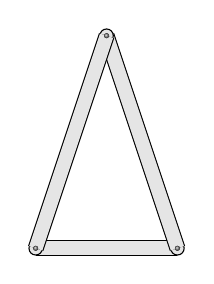
\begin{tikzpicture}[>=stealth,scale=0.9]
  \tkzSetUpPoint[fill=black]
  % \useasboundingbox(-1,-0.75)rectangle(3.7,1.4);
  \tkzDefPoints{-1/-3/B,1/-3/C,0/0/A}
  \draw[thin,double=gray!20,double distance=5pt](C)--(B);
  \filldraw[gray!20,thin,draw=black](B)circle(2.7pt);
  \filldraw[gray!20,thin,draw=black](C)circle(2.7pt);
  \draw[thin,double=gray!20,double distance=5pt](C)--(A);
  \filldraw[gray!20,thin,draw=black](A)circle(2.7pt);
  \draw[thin,double=gray!20,double distance=5pt](A)--(B);
  \fill[ball color=gray](A)circle(1pt);
  \fill[ball color=gray](B)circle(1pt);
  \fill[ball color=gray](C)circle(1pt);
\end{tikzpicture}
\end{document}